\documentclass{koala-en}
\usepackage[english]{babel}
\usepackage{lastpage}
\usepackage{pdfpages}
\renewcommand{\arraystretch}{1.5} %% Aeration des tableaux
\hyphenpenalty 10000
\usepackage{fancyhdr}
\usepackage{fmtcount}
\pagestyle{fancyplain}
\fancyhf{}
\renewcommand{\chaptermark}[1]{\markboth{#1}{}}
\renewcommand{\sectionmark}[1]{\markright{#1}}
\renewcommand{\headrulewidth}{0.8pt}
\renewcommand{\footrulewidth}{0.8pt}
\fancyhead[R]{\nouppercase{\leftmark}}
\lfoot{Camille Gardet - Internship report - August 2014}
\rfoot{\thepage/\pageref{LastPage}}
\setcounter{secnumdepth}{5}
\setcounter{tocdepth}{5}
\newcommand*{\glossaryname}{Dictionary}
\usepackage[numberedsection]{glossaries}
\newcommand{\dictentry}[2]{%
  \newglossaryentry{#1}{name=#1,description={#2}}%
  \glslink{#1}{#1*}%
}
\makeglossaries

%%%%%%%%%%%%%%%%%%%%%%%%%%%%%%%%%%%%%%%%%%%%%%%%

\begin{document}

\title{Internship report}
\subtitle{CS - from  May, \ordinalnum{5} to October, \ordinalnum{7}}

\member{Camille Gardet - }{camille.gardet@epitech.eu}

\summary
{
  This document contains three distinct sections, written in english, intended for three different kinds of person :
  \begin{itemize}
     \item The first is made for a newcomer in the company, it presents the project in which I was involved, very technically detailled to ensure a good ``getting started''.
     \item The second is a plea to my internship supervisor to fit into the team of a new project that I am particularly interested in.
     \item The last is a brief and non technical presentation to convince a high supervisor to entrust me with the full responsibility for a project, from start to finish, with customer contacts.
  \end{itemize}
In the structure of this document, words with a star in their right upper corner means that you can find a definition in the glossary at the end of this document. It's linked (only for numeric version, should I precise this ?).
  \newline
  \newline
  \newline
  \newline
  I would like to thank my supervisor \textbf{M. Thomas ANDREJAK} who supervised and mentored my work, for his attention and for all the time he spended on my work.
  \newline
  \newline
  I also thank the whole \emph{Prelude} team, consisting of \textbf{M. Gilles LEHMANN}, \textbf{M. Antoine LUONG}, \textbf{M. Avinash PARDESSY}, \textbf{M. Song TRAN}, \textbf{M. Enguerrand DE MAUDUIT}, \textbf{M. Jean-Charles ROGEZ}, \textbf{M. Thomas BURGUIERE} and \textbf{M. Vincent QUEMENER}, who were always here to help me.
}

\maketitle

\newpage
\thispagestyle{empty}

\tableofcontents

\clearpage
\thispagestyle{empty}
\newpage

\part{Documentation for a newcomer}
\chapter{Company presentation}
\section{Sector}
CS is an international company specialized in critical systems for target markets such as : defense, security, space, aeronautics and energy.

\begin{figure}[!ht]
  \center
  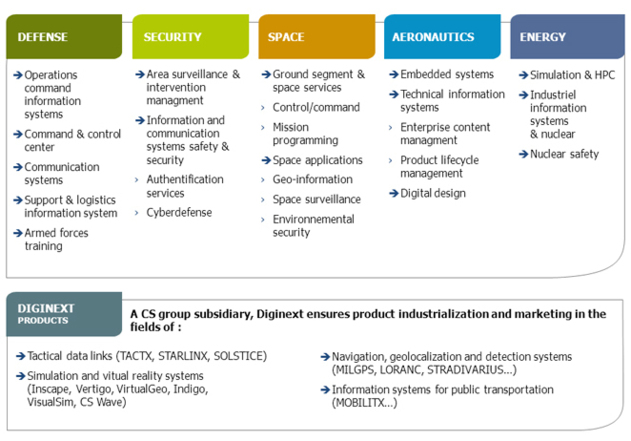
\includegraphics{market.jpg}
  \caption{Critical sectors}
\end{figure}

CS is now a leader in the field of air traffic control. Diginext, a subsidiary of the company, is a leader in \emph{\dictentry{Link 16}{A military tactical data exchange network used by US and NATO. Its specification is part of the family of Tactical Data Links}} and military data links. It provides software, hardware, logistics and ensure the maintenance in operational condition.

\section{Company}
CS has a worldwide influence, market, and has offices in France, Germany, Croatia, Romania, United-Kingdom, Chile, Canada, Emirates, US, Puerto Rico.

\begin{figure}[!ht]
  \center
  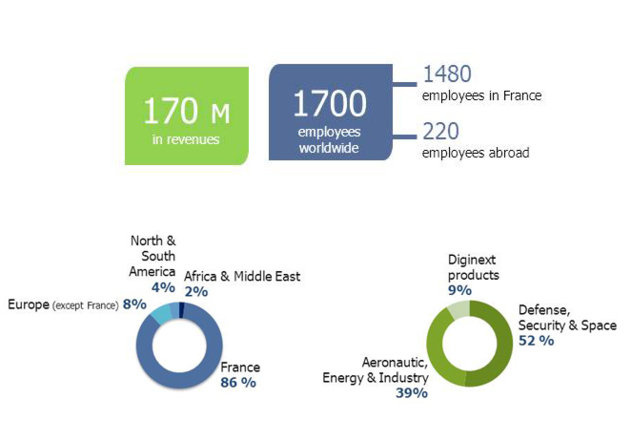
\includegraphics{revenue.jpg}
  \caption{International partners and turnover allocation}
\end{figure}

The company is in partnership with top-notch industrial and commercial company like EADS and Cegelec for air operations, Intel and Wolfram for high performance consulting, Sopra for logistics information systems.

\thispagestyle{fancy}
\newpage

\section{Business unit}

\begin{figure}[!ht]
  \center
  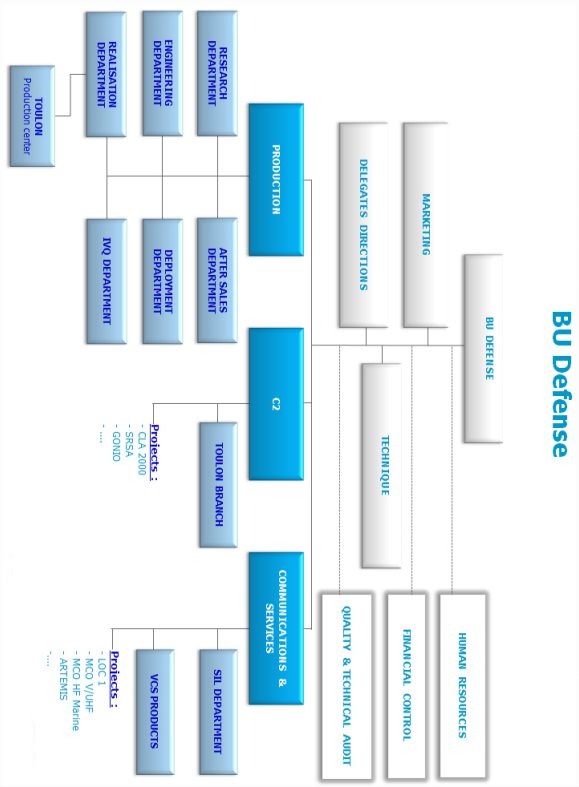
\includegraphics[width=15cm]{ochart.png}
  \caption{Organization chart of the Defense Business Unit}
\end{figure}

The mission of the Defense business unit is to implement solutions that meet the internal and external security needs, design and integrate command centers to collect, share and view in real time all the information needed for planning and driving joint army operations.

\section{Contextualization}
CS has a dual experience, on one hand in developing security components and solutions, and on the other hand, managing several e-administration and e-transaction projects. Moreover, with its strong expertise in cryptography and public key infrastructures, CS offers a complete range of security applications: encryption and implementation in networking equipment, identification and validation, non-reversible transactions, data and interchange confidentiality, secured application flows, and rights management and attribution.
\newline
\newline
In January 2012, CS acquires \emph{Prelude-IDS}, an open-source \dictentry{SIEM}{Security Information \& Event Management - Provide real-time analysis of security alerts generated by network hardware and applications}. An important goal for strategy development, it becomes a priority to rebuilt it, and put it back online. Targetting a emergent and promising martket for firm security, \emph{Prelude} could become a pioneer product.

\thispagestyle{fancy}
\newpage

\chapter{Prelude}
\section{Definition - What is Prelude ?}

\begin{figure}[!ht]
  \center
  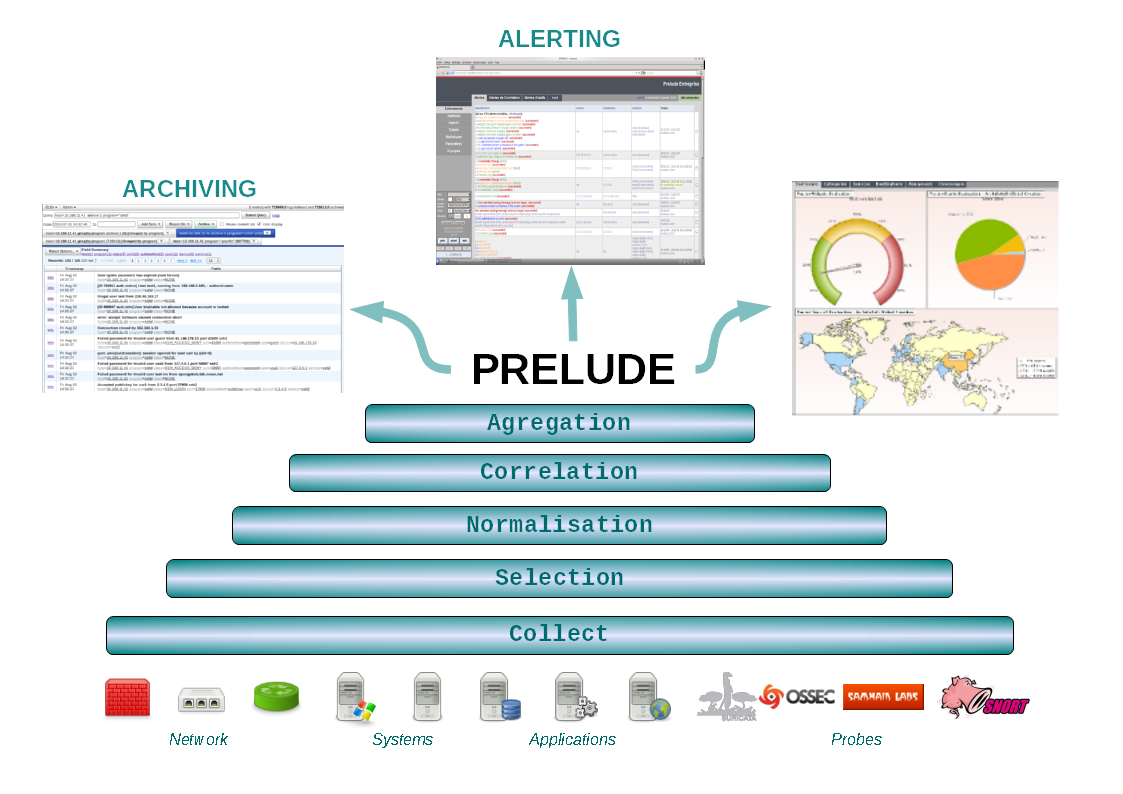
\includegraphics[width=15cm]{archi-simple.png}
  \caption{General overview}
\end{figure}

Prelude is a universal \emph{Security Information \& Event Management} (\dictentry{SIEM}{Security Information \& Event Management - Provide real-time analysis of security alerts generated by network hardware and applications}) system. Prelude collects, normalizes, sorts, aggregates, correlates and reports all security-related events independently of the product brand or license giving rise to such events.
\newline
\newline
As well as being capable of recovering any types of logs (system logs, syslog, flat files, etc.), Prelude benefits from a native support with a number of systems dedicated to enriching information even further (snort, samhain, ossec, auditd, etc.).
\newline
\newline
Security events are normalized into a single format, called the \emph{Intrusion Detection Message Exchange Format} (\dictentry{IDMEF}{Intrusion Detection Message Exchange Format - define data formats and exchange procedures for sharing information of interest to intrusion detection and response systems and to the management systems that may need to interact with them}). This format is an international standard format created upon the initiative of \dictentry{IETF}{Internet Engineering Task Force - develops and promotes voluntary Internet standards} along with the participation of Prelude team. It allows interaction with the various security tools currently available on the market.


\section{How does it work ?}

In figure 2.2, the different parts of the system and their interaction are illustrated.

\begin{figure}[!ht]
  \center
  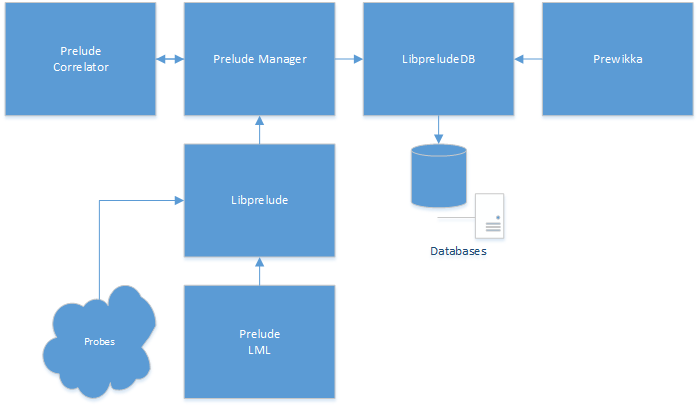
\includegraphics[width=15cm]{prelude.png}
  \caption{Communication between elements}
\end{figure}

\emph{Prelude-LML} is a log analyser that allows \emph{Prelude} to collect and analyze information from all kind of applications emitting logs or syslog messages in order to detect suspicious activities and transform them into Prelude-\dictentry{IDMEF}{Intrusion Detection Message Exchange Format - define data formats and exchange procedures for sharing information of interest to intrusion detection and response systems and to the management systems that may need to interact with them} alerts. \emph{Prelude-LML} handles alerts generated by a large set of applications.
\newline
\newline
\emph{Libprelude} is a library that guarantees secure connections between all sensors and the \emph{Prelude Manager}. \emph{Libprelude} provides an \dictentry{API}{Application Programming Interface - specifies how some software components should interact with each other} for the communication with \emph{Prelude} sub-systems, it supplies the necessary functionality for generating and emitting IDMEF alerts with \emph{Prelude} and automates the saving and re-transmission of data in times of temporary interruption of one of the components of the system.
\emph{Libprelude} also makes it easy for third party software to be made ``Prelude Aware'' (able to communicate with \emph{Prelude} components). This library provides common, useful features used by every sensors.
\newline
\newline
\emph{Prelude-Manager} is a high availability server that accepts secured connections from distributed sensors and/or other Managers and saves received alerts to a media specified by the user (database, log file, mail etc.). The server schedules and establishes the priorities of treatment according to the critical character and the source of the alerts.
The \emph{Prelude Manager} is a concentrator capable of handling large number of connections, and processing large amounts of alerts. It uses a per client scheduling queues in order to process alerts by severity fairly across clients.
The \emph{Prelude Manager} comes with multiple plugins like filtering plugins (idmef-criteria, thresholding, etc.) or reporting plugins like the \dictentry{SMTP}{Simple Mail Transfer Protocol - an Internet standard for electronic mail transmission} plugin which automatically sends emails containing a textual description of alerts to a configured list of recipients.
\newline
\newline
The \emph{LibpreludeDB} library provides an abstraction layer upon the type and the format of the database used to store IDMEF alerts. It allows developers to use the \emph{Prelude} IDMEF database easily and efficiently without worrying about \dictentry{SQL}{Structured Query Language - is a special-purpose programming language designed for managing data held in a relational database management system}, and to access the database independently of the type/format of the database.
\newline
\newline
The \emph{Prelude-Correlator} allows conducting multistream correlations thanks to a powerful programming language for writing correlation rules. \emph{Prelude-Correlator} is a Python rules based correlation engine. It has the ability to connect and fetch alerts from a remote \emph{Prelude-Manager} server, and correlate incoming alerts based on the provided ruleset. Upon successful correlation, IDMEF correlation alerts are raised.
\newline
\newline
\emph{Prewikka} is the \dictentry{GUI}{Graphical user interface - type of interface that allows users to interact with electronic devices through graphical icons and visual indicators such as secondary notation, as opposed to text-based interfaces, typed command labels or text navigation} of \emph{Prelude}. Web-based, it shows alerts, correlated alerts, probes states, statistics about systems, alerts, and so on.

\chapter{Latest developments - Documentations}
Prelude is an old and open-source project without any user or developer documentations.
\newline
\newline
A part of my mission was to write these documentations. My work was guided by the reference documents, made by CS team previous user :
\begin{itemize}
  \item System/Subsystem Specification (SSS) - The requirements to be met by the system,
  \item System/Subsystem Design Description (SSDD) - The design of the system
\end{itemize}

The first and second sections of this chapter are dedicated to present these documents, and the modifications I made.
\newline
The final documentation should cover all the modules of \emph{Prelude}. The documentation must follow the standards defined by CS so, guidelines to write these documents are provided below. And to illustrate my words, I use \emph{Libprelude} documentation, already written, as an example.

\thispagestyle{fancy}
\newpage

\section{System/Subsystem Specification (SSS)}
The SSS lists all the requirements that the documentation must follow.

\subsection{Needs}
Understanding the needs is one of the first thing to know and answer questions like \emph{Why do I need this ?} or \emph{How can I fulfill this requirements ?}. The requirements are submited by the client, most of time, but also by CS, to match intern standard.

\subsection{Technical requirements}
\emph{How things should work ?}
\newline
While being general, each features of a module are formated as a requirement, describing its operating.
A small flow-chart to illustrate this is strongly recommended.

\begin{figure}[!ht]
  \center
  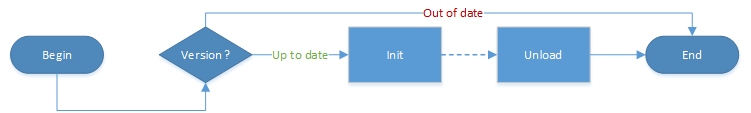
\includegraphics[width=15cm]{sss.png}
  \caption{Loading Libprelude - How should it proceeds}
\end{figure}

Followed by :

\begin{lstlisting}
  LIB_USE_VERSION : Check library version
  How : Use a function to return the version
  Why : The version must be checked before the initialisation

  LIB_INIT...

  LIB_UNLOAD...
\end{lstlisting}

\subsection{External interface requirements}
\emph{What will provide external connection ?}
\newline
Not only network of course. Everything that will communicate with the module is an external interface.
It can be others modules of the project, or an external library, or an \dictentry{API}{Application Programming Interface - specifies how some software components should interact with each other}, or a language binding, etc.

\subsection{Internal interface requirements}
\emph{What use my module to run properly ?}
\newline
If the module uses a configuration file, or data in a specified standard format, it should be listed as an internal interface. For example, the IDMEF format is specified in a \dictentry{RFC}{Request For Comments - the principal technical development and standards-setting bodies for the Internet}.

\subsection{Environment requirements}
List everything environment related, like \emph{Should my library be crossplatform ?} or \emph{What happens when my system reboot ?}.

\subsection{Definition and conception constraints}
Languages or tools that \textbf{must} be used to implement the module. \emph{Libprelude} must be written in C for example.

\section{System/Subsystem Design Description (SSDD)}
\subsection{Design principle}
Every main parts of the module must have a description of how it will be designed. This description can be data exchange, communication channel or error and configuration management.

\subsection{Software structure}
\emph{What is the internal structure ?}
\newline
It can be a tree view, with details about folders, what it contains, why is it used. Third-party library are also mentioned here, with proper explanations given on its usage.

\subsection{System operating}
This is the most detailled part of the documentation. The unit of scale is the function and it describes what does it do, and how it does it. All the functions of all parts of the module must be listed and fully documented.
\newline
\newline
Short example for \emph{Libprelude} and the function to initialise the library in figure 3.2.

\begin{figure}[!ht]
  \center
  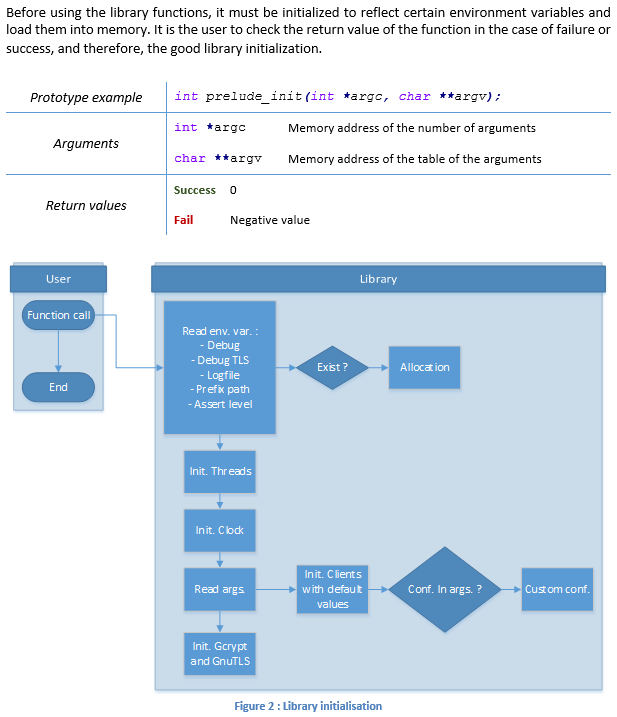
\includegraphics{sysop.png}
  \caption{Description of the library init function in Libprelude}
\end{figure}

\thispagestyle{fancy}
\newpage

\chapter{Latest developments - Coding}
In this chapter, I list the CS standard and the latest development I made.

\section{CS standard}
To develop features on \emph{Prelude}, CS recommends to use :
\begin{itemize}
  \item CentOS 6 virtual machine,
  \item Python 2.6,
  \item C, standard C89,
  \item Redmine, for project management and bug-tracking tool,
  \item Latest version of Prelude, found on \url{http://www.prelude-ids.org}
\end{itemize}

\section{A new probe, Motion}
The latest development is about image detection. \emph{How to combine a webcam and the probe to raise alert of movements detection ?}

\subsection{Motion ?}
Motion is a small tool to monitor video streams, coming from one or many video devices and is able to detect movement.
\newline
\newline
The tool is written in C for linux based OS.
\newline
\newline
Since its version 3.1.12, the tool is maintained by Kenneth Lavrsen and a small community.
\newline
Homepage : \url{http://www.lavrsen.dk/foswiki/bin/view/Motion/WebHome}

\subsection{Implementation}
The motion source code is well commented. It is easy understandable.
\newline
\newline
The files \emph{motion.c} and \emph{motion.h} contains the code that allow movements detection. An alert is raised from these files.
\newline
\newline
Motion uses a structure \emph{context} which includes the whole software configuration during its execution, and the last recorded pictures.
Prelude initialisation is done at the initialisation of this structure :
\begin{lstlisting}
  AlertPreludeCtx *prelude_ctx = AlertPreludeInitCtx();
  cnt->prelude_context = prelude_ctx;
\end{lstlisting}
The function \emph{AlertPreludeInitCtx()} initialises a Prelude context.
\newline
\newline
The function \emph{motion\_loop()} is a infinite loop to capture the video stream, and detects a movement. The alert-raising code is inserted in :
\begin{lstlisting}
  AlertPrelude(cnt->prelude_context, cnt->current_image);
\end{lstlisting}
The function \emph{AlertPrelude()} creates and sends an alert to the \emph{Prelude Manager} with the current image as extra data, to be able to display it for example.

\subsection{Results}
After registering Motion in Prelude and running it, it appears as a probe in \emph{Prewikka}, as illustrated in figure 4.1.
\begin{figure}[!ht]
  \center
  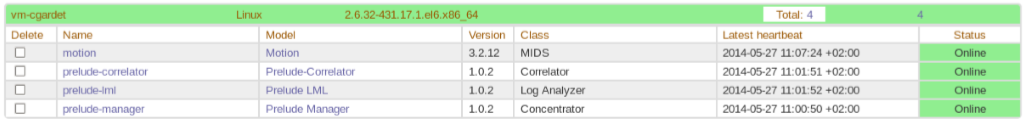
\includegraphics[width=15cm]{motionprobe.png}
  \caption{Motion as a probe in Prewikka}
\end{figure}

And it generates some alerts as well. An example of alerts raised by Motion \emph{Prewikka} is available in figure 4.2.
\begin{figure}[!ht]
  \center
  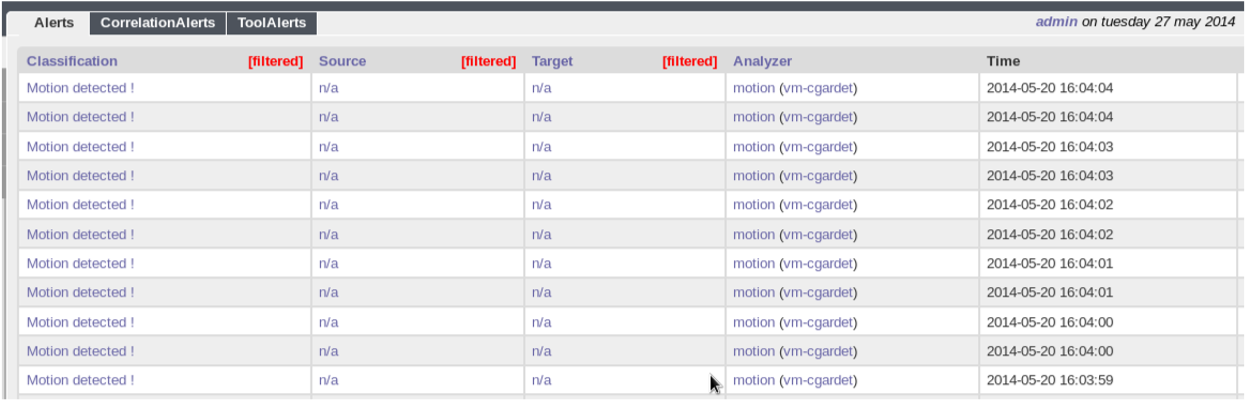
\includegraphics[width=15cm]{motionalerts.png}
  \caption{Alerts raised by Motion in Prewikka}
\end{figure}

The version of \emph{Motion} with \emph{Prelude} patch is provided in the link in the appendix.

\thispagestyle{fancy}
\newpage

\section{Enhance statistics in Prewikka}
A part of my work was to create new visualisation graph to diversify statistics / forensics.

\subsection{One library, to rule them all}
Old graphs are Adobe Flash based, an ageing technology.
\newline
\newline
Instead, Javascript is recommended in this case and already used in \emph{Prewikka}. After a small research, the library \textbf{D3.js} seems to fulfill all the needs.
\newline
\newline
\emph{D3} binds arbitrary data to a Document Object Model (DOM), and then apply data-driven transformations to the document. For example, \emph{D3} generates an HTML table from an array of numbers, or uses the same data to create an interactive SVG bar chart with smooth transitions and interactions.
\newline
\newline
Homepage : \url{http://d3js.org/}
\newline
Example gallery : \url{https://github.com/mbostock/d3/wiki/Gallery}

\subsection{Implementation}
For any graph, the first step is creating a standalone version, working offline, supplied from a CSV data file. Data can be IDMEF fields like :
\begin{lstlisting}
``IP Source'', ``IP Target'', ``Assessment'', ``Analyzer'', ``Date''
``10.10.10.3'',''232.136.239.176'',''Bruteforce'',''Prelude-LML'',''24/02/2005T11:45''
``10.10.10.20'',''193.227.171.216'',''SSH Failed'',''Snort'',''09/02/2005T14:59''
``10.10.10.16'',''106.190.182.175'',''SSH Failed'',''OSSEC'',''09/10/2007T09:06''
\end{lstlisting}

Each line is an alert. A python script to generate this kind of file is provided in appendix.
\newline
\newline
Once the graph works, the integration in \emph{Prewikka} can begin. It means :
\begin{itemize}
  \item Templating - HTML code,
  \item Create view - Setting up data to fill the template,
  \item Fetch database - Collecting alerts from the database, and not from a file
\end{itemize}

Features already provided by \emph{Prewikka} must be kept, as filtering by date, event, etc.

\thispagestyle{fancy}
\newpage

\subsection{Results}
As example, a \dictentry{Circos}{Kind of graph to visualize data in a circular layout, ideal for exploring relationships between objects or positions. Homepage : \url{http://circos.ca/}}-like in D3.js. A scheme resume is provided in figure 4.3 and then an explanation about a detailed link in figure 4.4.

\begin{figure}[!ht]
  \center
  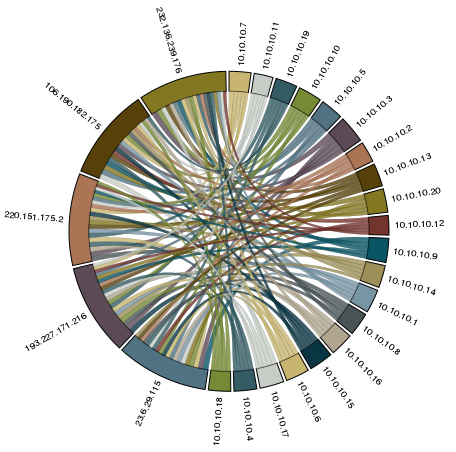
\includegraphics[width=15cm]{circos.png}
  \caption{Standalone version of a Circos-like graph}
\end{figure}

This chart is the resume of all the alerts, linked between two attributes. Here are the IP of the alert's target, beginning with ``10.'', and the IP of the alert's origin. A link between two groups represents an alert, and its information can be view by hovering the mouse on it, or on a group (figure 4.4).

\begin{figure}[!ht]
  \center
  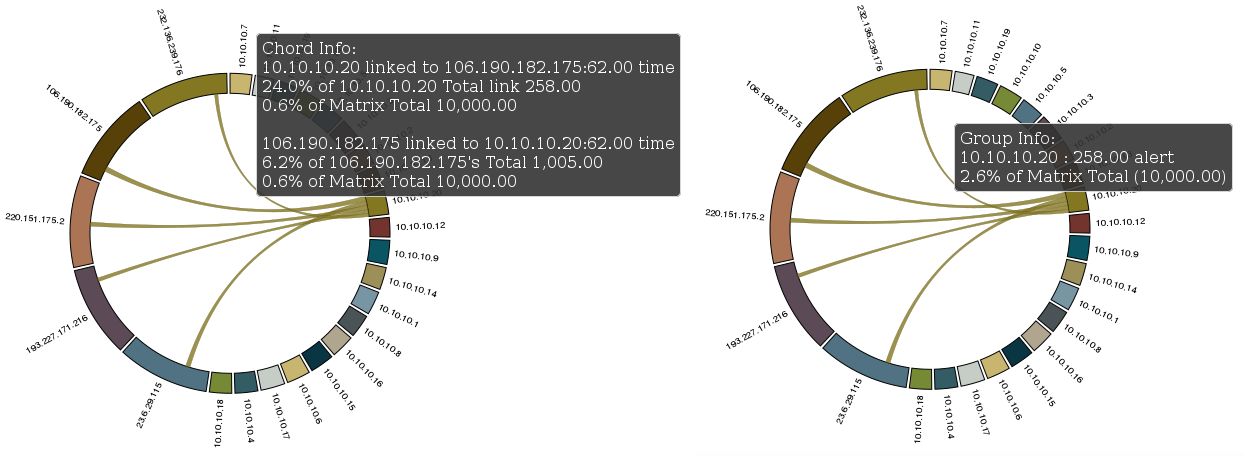
\includegraphics[width=15cm]{circostt.png}
  \caption{More information about links}
\end{figure}

\thispagestyle{fancy}
\newpage

The merge of the standalone version in the \emph{Prewikka} code with the filters can be done. Few modifications must be made to apply correctly the filters provided in the GUI, and to modify in real-time the graph.
\newline
A new ``Forensic'' menu is made where the type of the graph is created under a new tab with its name and where the others graphs should be added.

\begin{figure}[!ht]
  \center
  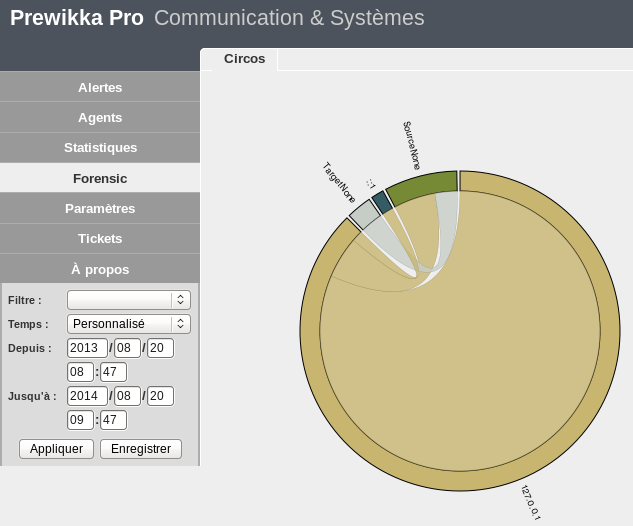
\includegraphics[width=15cm]{circosprew.png}
  \caption{The graph in \emph{Prewikka}}
\end{figure}

\thispagestyle{fancy}
\newpage

\section{Make GeoIP customisable}
\subsection{GeoIP ?}
\emph{GeoIP} enables the identification, the location, organization, connection speed, and user type of an IP address. The GeoIP databases are among the most popular and accurate IP geolocation databases available.
\newline
\newline
Homepage : \url{https://www.maxmind.com}
\newline
\newline
It is used in \emph{Prelude} to locate the origin of an alert.

\subsection{Implementation}
\emph{Customisable ?}
Actually, only public IP addresses can be identified, which is how the tool performs. It might be possible to create custom IP ranges and to associate them to a custom location.
\newline
\newline
\emph{How GeoIP works ?} Ranges of IP are stored in a database and linked to a location. E.g. : 2.0.0.0 to 2.15.255.255 are reserved to \emph{France Telecom}. Knowing this, it is easy to compare and get the location name of a determined IP. This IP database is highly optimized, not directly readable and \emph{Maxmind} does not provide tools to modify it. So, in this approach the first step is finding a way to decypher it, then insert custom ranges, and finally re-cypher it. However, the database exists in a CSV file format, avoiding the decyphering step, and implying a regeneration of the database binary formated.
\newline
\newline
As for the description of the graphs, a view and a template must be created. The template is a simple HTML form with the necessary fields to fill up a custom range. The view is python code to parse the GeoIP CSV file and to store it in a dictionnary. The file is provided in the appendix.

\subsection{Results}
As seen in figure 4.6, the form displays four commands :
\begin{itemize}
  \item ``Create a range''. Allows the creation of a location with its long name and associates it a two letters short name.
  \item ``Select a range''. Loads or Deletes an existing range. If loaded, the range displays the IP in the field ``IP Range''.
  \item ``IP range''. Shows all the IP ranges of the selected location, with the possibility to massive deletion/insertion and submit a modification,
  \item ``Export to GeoIP binary file''. Converts the CSV file format to binary database, used by all the API provided by \emph{Maxmind}
\end{itemize}

\begin{figure}[!ht]
  \center
  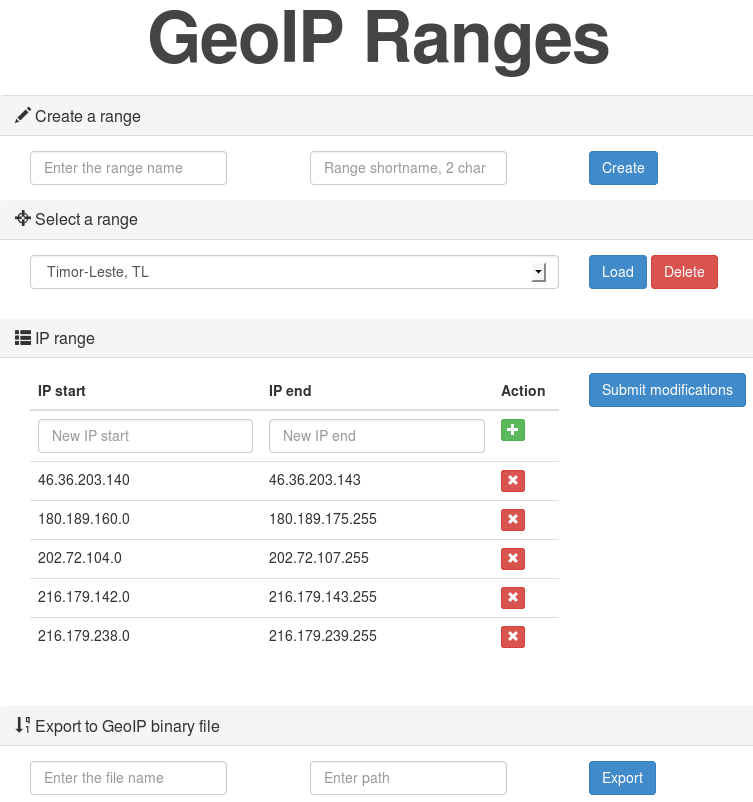
\includegraphics[width=15cm]{geoip.png}
  \caption{The form to create/edit/delete GeoIP range}
\end{figure}

\chapter{Final word}

Working on this kind of project is challenging. The documentation improves your knowledge about the system, but also the standard requirements for documentation writing. The IDMEF format is unfortunately barely used, but tends toward to be used. Technically, both old and new languages are used, C, Python, SQL, JavaScript, making \emph{Prelude} an all-round project.
\newline
\newline
Personnaly, I wish to join the \emph{Prelude} team and continue working on the enhancement and modernization of the project.

\thispagestyle{fancy}
\newpage

%% Lexicon
\printglossary[style=altlisthypergroup]
\thispagestyle{fancy}

\chapter{Appendix}

All of the files can be viewed on \url{https://github.com/M3nace/Prelude}

\section{Python script to generate alert}
\begin{lstlisting}
#!/usr/bin/env python3
"''
Generate alert and store them in a CSV file, formated like :
``target'', ``source'', ``classification'', ``analyzer'', ``date'',
    ^           ^               ^                ^            ^
    |           |               |                |            |
    |           |               |                |            --------- The date of the alert, format : DD/MM/YYYYTHH:MM
    |           |               |                |
    |           |               |                ------------------- Analyzer name, which create the alert
    |           |               |
    |           |               ----------------------------------- Type of the alert
    |           |
    |           ------------------------------------------------ IP of the device which create the alert
    |
    ---------------------------------------------------------- IP of the device which has been targeted

Contiguous IP are generated with the function ipRange(start, end), to simulate a targeted network.
Where ``start'' is the first IP in the range and ``end'', the last. Both type are strings.
E.g. : ipRange(``192.168.1.0'', ``192.168.1.5'') will return a list including :
[ ``192.168.1.0'', ``192.168.1.2'', ``192.168.1.3'', ``192.168.1.4'', ``192.168.1.5'' ]

Random date are generated with the function randomDate(start, end), to simulate attacks on a period of time.
Where ``start'' is the beginning of a period, and ``end'', the end of it. Both type are datetime.

IP Source are randomly generated and stored in a list.
Classification and analyzer are randomly picked from an established list. Lazy, I know.

And finally, the CSV is written, line by line, picking a ``random'' settings each loop. ``Random'' because
the random module should be called ``pseudo-random'':
> Generate 5000 alerts.
> You have a list of 5 analyzers.
> You will have a CSV where each analyzer appears around 1000 times.
> That's not a place to talk about that.
"''

import os
import sys
import random
import csv
import json
import time
from datetime import timedelta
from datetime import datetime
from random import randint

# How many IP source do you want ?
nb_ip_source = 5
# How many alert (line in the CSV file) do you want ? /!\ The higher, the harder to compute (for the diagram) /!\
nb_alert = 5000

def ipRange(start_ip, end_ip):
   start = list(map(int, start_ip.split(``.'')))
   end = list(map(int, end_ip.split(``.'')))
   temp = start
   ip_range = []

   ip_range.append(start_ip)
   while temp != end:
      start[3] += 1
      for i in (3, 2, 1):
         if temp[i] == 256:
            temp[i] = 0
            temp[i-1] += 1
      ip_range.append(``.''.join(map(str, temp)))

   return ip_range


def randomDate(start, end):
   return (start + timedelta(seconds=randint(0, int((end - start).total_seconds())))).strftime('%d/%m/%YT%H:%M')#.date()


def main(argv=None):
   target_list = ipRange(``10.10.10.1'', ``10.10.10.20'')
   source_list = [ ]
   classification_list = [ ``SSH Failed'', ``Bruteforce'', ``DDoS'', ``Eth. Sniffing'', ``Buffer overflow'' ]
   analyzer_list = [ ``Prelude-LML'', ``Suricata'', ``OSSEC'', ``Samhain'', ``Snort'' ]
   date_begin = datetime.strptime(``01 Jan 00'', ``%d %b %y'')
   date_end = datetime.strptime(``31 Dec 14'', ``%d %b %y'')
   # We list the index here, to write it on the first line of the CSV file
   indexes = [``target'', ``source'', ``classification'', ``analyzer'', ``date'']

   for j in range(nb_ip_source):
      source_list.append('.'.join('%s'%random.randint(0, 255) for i in range(4)))

   with open('alert.csv', 'w') as csvfile:
      spamwriter = csv.writer(csvfile, delimiter=',', quotechar='''', quoting=csv.QUOTE_ALL)
      spamwriter.writerow(indexes)
      for i in range(nb_alert):
         spamwriter.writerow([random.choice(target_list),
                              random.choice(source_list),
                              random.choice(classification_list),
                              random.choice(analyzer_list),
                              randomDate(date_begin, date_end)])

   return 0

if __name__==''__main__'':
   status = main()
   sys.exit(status)
\end{lstlisting}

\section{Python script to parse GeoIP CSV file}
\begin{lstlisting}
#!/usr/bin/env python

"''
CSVReader - Read a data.cvs GeoIP format file and store it in a dictionary
The CVS format parsed must match the GeoIPCountryWhoIs.cvs :
``IP Start'', ``IP End'', ``IP Start INT format'', ``IP End INT format'', ``Short Name'', ``Range Name''
    -> IP Start/End : the first/last ip of the range
    -> IP Start/End INT format : Same as IP start, but in int format (see below)
    -> Short Name : Abreviation for the range name
    -> Range Name : Full range Name
Example : ``192.168.1.0'', ``192.168.1.255'', ``3232235776'', ``3232236031'', ``SN'', ``Small Network''

IP int calculation :
(first octet * 256^3) + (second octet * 256^2) + (third octet * 256) + (fourth octet)
For 192.168.1.0 :
    (192 * 256^3) + (168 * 256^2) + (1 * 256) + (0)
<=> 3221225472 + 11010048 + 256
<=> 3232235776

The dictionary keys are the tuple (Range Name, Short Name)
The items are a list of as many tuple as IP range for the key
Example :
(Private Network, PN)
[
    (``10.0.0.0'', ``10.255.255.255'', ``167772160'', ``184549375''),
    (``172.16.0.0'', ``172.31.255.255'', ``2886729728'', ``2887778303''),
    (``192.168.0.0'', ``192.168.255.255'', ``3232235520'', ``3232301055'')
]

(My Network, MN) [(``127.3.0.0'', ``127.3.255.255'', ``2130903040'', ``2130968575'')]
"''

import csv
import collections

class CSVReader:
    def __init__(self, csv_file):
        self.csv_file = csv_file
        self.db = { }

    def parse_file(self):
        with open(self.csv_file, 'r') as fd:
            reader = csv.reader(fd)
            for row in reader:
                ip_start, ip_end, ipint_start, ipint_end, short_name, range_name = row
                if (range_name, short_name) in self.db:
                    self.db[(range_name, short_name)] += [(ip_start, ip_end, ipint_start, ipint_end)]
                else:
                    self.db[(range_name, short_name)] = [(ip_start, ip_end, ipint_start, ipint_end)]

        self.db = collections.OrderedDict(sorted(self.db.items()))

    def delete(self, range_name):
        if range_name in self.db:
            del self.db[range_name]

    def create(self, range_name):
        self.db[range_name] = None

    def insert_ip(self, range_name, value):
        if range_name in self.db:
            self.db[range_name] += value
        else:
            self.db[range_name] = value

    def write_csv(self):
        with open(self.csv_file, 'wb') as fd:
            writer = csv.writer(fd, delimiter=',', quotechar='''', quoting=csv.QUOTE_ALL)
            for key, ip_lists in self.db.iteritems():
                for ip_range in ip_lists:
                    ip_start, ip_end, int_start, int_end = ip_range
                    range_name, range_short = key
                    writer.writerow([ip_start, ip_end, int_start, int_end, range_short, range_name])

    def get_range(self):
        return self.db.keys()

    def get_ip_from_range(self, range_name):
        if range_name in self.db:
            return self.db[range_name]
        else:
            return [ ]

    def get_whole_db(self):
        return self.db

\end{lstlisting}

\thispagestyle{fancy}

\part{Letter to my internship supervisor}
Dear Sir,
\newline
\newline
I am particularly interested in the new position into the Prelude team.
\newline
\newline
During my six months internship, I enhance the documentation of the project. It gives me the necessary knowledge to develop the requested new features, and I am able to create new probe for \emph{Prelude}.
\newline
Developing these features also gives me the understanding in the detailed mechanics of the project, and the assimilation of the CS standards, which allows me to work faster and the same way as the others members of the team. Not to mention the social interactions with the team, that facilitate my integration.
\newline
\newline
This internship comforts me in the idea of continuing in the team at the end of my studies, if possible.
\newline
\newline
To talk about this position and, I hope, of my future job at CS, I would like to have a meeting with you.
\newline
\newline
Thank you for your time and consideration.
\newline
\newline
Best regards,\newline
Camille Gardet

\thispagestyle{fancy}

\part{Letter to a high supervisor}
Dear Sir,
\newline
\newline
I am currently finishing a six months internship working on \emph{Prelude}, during which I develop my skills on several topics. It was mostly technical, but I got a glimpse of the managerial side of those topics.
\newline
\newline
Thanks to an efficient and warm integration of the others members of \emph{Prelude}, my work reaches the require standards of CS and
is added in the project. I had the chance to take part of the last congress, where \emph{Prelude} was showed, which allows me to have several contacts with potential customers.
\newline
Also, I have good feedbacks on my work despite the fact that I had a limited time, to take hand on the tools to do my job. I sincerely believe that I am able to learn to manage a project in a short time, and so, I am able to have a complete responsibility on a project. My thoughts are also based on the fact, that I already did it at school during 5 years. I was the leader of small groups of students for several projects involving team management.
\newline
\newline
Many contracts will signed at the beginning of the year. I am particularly interested in one of them.
\newline
\newline
To talk about this position and, I hope, of my future job at CS, I would like to have a meeting with you.
\newline
\newline
Thank you for your time and consideration.
\newline
\newline
Best regards,\newline
Camille Gardet

\thispagestyle{fancy}
\end{document}
